\subsection{Opgave 22}

En vektor $\Vec{a}$ er bestemt ved
\begin{align*}
    \Vec{a} = \begin{pmatrix}5\cdot \cos(60^{\circ}) \\ 5\cdot \sin(60^{\circ})\end{pmatrix}
\end{align*}
Forklar hvad tallene 5 og $60^{\circ}$ fortæller om $\Vec{a}$\\\\

\ans
Tallet 5 fortæller os at $\Vec{a}$ har længden 5. Tallet $60^{\circ}$ er vektorens retningsvinkel altså den vinkel der er mellem vektoren og x-aksen. Dette kan ses illustreret på følgende graf\\\\
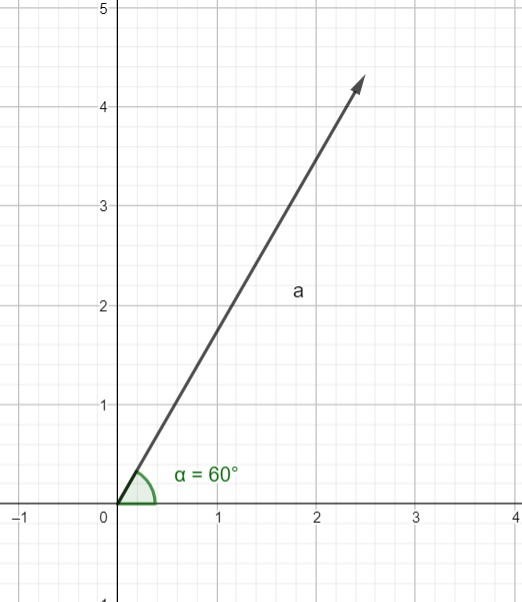
\includegraphics[width = 6cm]{Opgave_21-30/Opgave_22/22.jpg}